\documentclass[14pt,a4paper]{extreport}
\usepackage[utf8]{inputenc}
\usepackage{mathptmx}
\usepackage{graphicx}
\usepackage{geometry}
\geometry{a4paper, margin=1in}
\usepackage{setspace}
\usepackage{titlesec}
\usepackage{tocloft}
\usepackage{float}
\usepackage{hyperref}

% To match the template's lack of chapter numbering in titles or specific styling
\titleformat{\chapter}[display]
  {\normalfont\fontsize{14}{18}\selectfont\bfseries}{\chaptertitlename\ \thechapter}{10pt}{\fontsize{14}{18}\selectfont\bfseries}
\titleformat{\section}
  {\normalfont\fontsize{14}{18}\selectfont\bfseries}{\thesection}{10pt}{\fontsize{14}{18}\selectfont\bfseries}
\titleformat{\subsection}
  {\normalfont\fontsize{14}{18}\selectfont\bfseries}{\thesubsection}{10pt}{\fontsize{14}{18}\selectfont\bfseries}
\titlespacing*{\chapter}{0pt}{-50pt}{20pt}

% Ensure Table of Contents title matches the 14pt chapter headings
\renewcommand{\cfttoctitlefont}{\normalfont\fontsize{14}{18}\selectfont\bfseries}
\renewcommand{\cftaftertoctitle}{}

\begin{document}

\begin{titlepage}
    \begin{center}
        \vspace*{0.5cm}
        
        \fontsize{20}{24}\selectfont
        \textbf{SmartEvent AI} \\
        \fontsize{14}{18}\selectfont
        \textbf{A Serverless Event Management Platform with WebRTC QR Verification} \\
        \vspace{0.8cm}
        \fontsize{14}{18}\selectfont
        A Report Submitted in \\
        Partial Fulfilment for \\
        award of Bachelor of Technology/Master of Integrated Technology \\
        \vspace{0.8cm}
        In \\
        \textbf{Web Technologies (BCSE0455/ BCSEH0455/BMICSE0455)} \\
        \fontsize{16}{20}\selectfont
        \textbf{COMPUTER SCIENCE} \\
        \fontsize{14}{18}\selectfont
        \vspace{0.8cm}
        By \\
        \textbf{Ashutosh Singh (2401330120038)} \\
        \textbf{Aniruddha Badani (2401330120025)} \\
        \textbf{Divyansh Verma (2401330120056)} \\
        
        \vspace{0.8cm}
        Under the Supervision of \\
        \textbf{Mr. Anshul Varshney} \\
        Assistant Professor \\
        
        \vspace{0.6cm}
        
\includegraphics[width=0.35\textwidth]{screenshots/niet_logo.png} \\
        \vspace{0.6cm}
        
        \fontsize{14}{18}\selectfont
        Department of Computer Science \\
        School of Computer Science and Information Technology \\
        \textbf{NOIDA INSTITUTE OF ENGINEERING AND TECHNOLOGY} \\
        GREATER NOIDA \\
        (An Autonomous Institute) \\
        Affiliated to \\
        DR. A.P.J. ABDUL KALAM TECHNICAL UNIVERSITY, LUCKNOW
        
    \end{center}
\end{titlepage}

\pagenumbering{roman}
\chapter*{DECLARATION}
\addcontentsline{toc}{chapter}{Declaration}
I hereby declare that the work presented in this report was carried out by me. I have not submitted the matter embodied in this report for the award of any degree or diploma of any other University or Institute.

\vspace{2cm}
\noindent
Team Leader: \\
Ashutosh Singh (Roll No.: 2401330120038) \\
\vspace{1cm}\\
\rule{5cm}{0.4pt} \\
(Candidate's Signature)

\vspace{1cm}
\noindent
Team Members: \\
1.) Aniruddha Badani (Roll No.: 2401330120025) \\
\vspace{1cm}\\
\rule{5cm}{0.4pt} \\
(Candidate's Signature)

\vspace{1cm}
\noindent
2.) Divyansh Verma (Roll No.: 2401330120056) \\
\vspace{1cm}\\
\rule{5cm}{0.4pt} \\
(Candidate's Signature)


\chapter*{CERTIFICATE}
\addcontentsline{toc}{chapter}{Certificate}
Certified that Ashutosh Singh (2401330120038), Aniruddha Badani (2401330120025) and Divyansh Verma (2401330120056) has carried out the project work presented in this Project Report in partial fulfillment of the requirements for the award of Bachelor of Technology/Master of Integrated technology, CSE(R) 2nd Year, 4th Sem from Noida Institute of Engineering \& Technology under my supervision.

\vspace{3cm}
\noindent
\begin{minipage}{0.5\textwidth}
Signature: \rule{4cm}{0.4pt} \\
\textbf{Mr. Anshul Varshney} \\
Assistant professor \\
Dept of Computer Science \\
NIET, Gr. Noida
\end{minipage}
\begin{minipage}{0.5\textwidth}
Signature: \rule{4cm}{0.4pt} \\
\textbf{Dr. Arun Kumar Tripathi} \\
Professor \& HOD \\
Dept. of Computer Science \\
NIET, Gr. Noida
\end{minipage}


\chapter*{ACKNOWLEDGEMENT}
\addcontentsline{toc}{chapter}{Acknowledgement}
I would like to express my heartfelt gratitude to Mr. Anshul Varshney for his invaluable guidance, support, and constant supervision throughout the development of this project. His expertise and encouragement have been pivotal in shaping the project.

I would also like to extend my thanks and appreciation to our esteemed HOD (Dr. Arun Kumar Tripathi) for his continuous motivation and support. His encouragement has been instrumental in completing this project successfully.

Finally, I am deeply thankful to my peers and everyone who directly or indirectly contributed to this project with their knowledge, advice, and assistance.


\chapter*{ABSTRACT}
\addcontentsline{toc}{chapter}{Abstract}
SmartEvent AI is a comprehensive serverless event management platform designed to streamline the organization, discovery, and administration of events. Developed using Vanilla HTML/CSS/JS and integrated with Firebase (Auth and Firestore), the platform provides real-time event status updates, a dynamic registration workflow, and role-based access control for students, organizers, and administrators. Key features include an intuitive dashboard, interactive charting for analytics, and a built-in WebRTC-based QR scanner for seamless attendance tracking. The platform emphasizes a modern, responsive user interface with a dark-mode aesthetic and zero-latency state synchronization. By replacing traditional monolithic architectures with a serverless paradigm, SmartEvent AI ensures high scalability and low maintenance overhead, serving as a robust solution for institutional and public event management.


\clearpage
\tableofcontents
\clearpage
\pagenumbering{arabic}

\chapter{INTRODUCTION}
\section{Overview}
In the modern educational and professional landscape, organizing, managing, and tracking attendance for events represents a significant administrative challenge. Traditional methods relying on manual spreadsheets or physical tick-sheets are highly prone to errors, scale poorly, and fail to provide immediate, actionable feedback to either organizers or attendees.

SmartEvent AI is a cutting-edge web-based event management platform designed to address these challenges. Operating on a modern Single Page Application (SPA) model, the platform delivers a fast, fluid, and responsive user experience. It leverages Backend-as-a-Service (BaaS) technologies via Firebase (Authentication and Cloud Firestore) to achieve real-time synchronization of event registration data, seat availability, and attendance logs across all active clients. The system is engineered to manage the entire lifecycle of an event: from dynamic creation and categorization to public self-registration, reactive digital ticket generation, and instantaneous on-site attendance verification using WebRTC-enabled camera QR code scanning.

\section{Objective And Scope}
\subsection{Objectives}
The primary objectives of the SmartEvent AI project are as follows:
\begin{itemize}
    \item \textbf{Eliminate Registration Friction:} Provide a seamless, self-service portal where users can discover upcoming events, track real-time seat counts, and register with a single click.
    \item \textbf{Enable Real-Time Administration:} Equip organizers and administrators with live-updating dashboards that display key operational metrics (e.g., ticket sales, category distribution, total revenue) using interactive charts without requiring page reloads.
    \item \textbf{Streamline On-Site Attendance:} Design and implement a zero-hardware attendance solution that permits organizers to use their mobile or desktop webcams to scan and validate digital tickets on the fly.
    \item \textbf{Implement Scalable Serverless Infrastructure:} Build the application entirely on serverless cloud systems to minimize host management overhead, maximize resource utilization, and scale effortlessly to hundreds of concurrent users.
\end{itemize}

\subsection{Scope}
The scope of this project encompasses:
\begin{itemize}
    \item A robust user authentication module supporting secure email/password and third-party Google OAuth credentials.
    \item Dynamic role-based user dashboards tailored specifically for Students (attendees), Organizers (event managers), and Administrators (global managers).
    \item Client-side state synchronization governed by a reactive pub/sub architecture (`SmartStore`) linked to real-time Firestore listeners.
    \item A secure database structure enforced via strict Firebase Security Rules that support organizational role reads.
    \item An integrated camera-based QR code parser utilizing the device's video stream through WebRTC and the client-side `jsQR` library.
\end{itemize}

\chapter{LITERATURE REVIEW}
\section{Overview of Existing Systems}
Existing event management architectures can generally be categorized into two paradigms: legacy monolithic enterprise portals and modern, highly integrated SaaS platforms (such as Eventbrite or Meetup). 

Monolithic applications typically rely on heavy server-side languages (like PHP, Java Spring, or ASP.NET) connected to local relational databases (MySQL, PostgreSQL). These systems process and render all logic on the server, generating static HTML pages that must be sent over the wire for every interaction. While highly stable, they suffer from high latency during traffic spikes and require extensive hardware provisioning to absorb temporary registration surges.

Integrated SaaS platforms leverage cloud networks and modern APIs, providing polished user interfaces and scalable backends. However, they are often closed-ecosystem platforms that charge steep transaction fees, offer limited direct customizability, and lack lightweight, offline-ready local scanning features out of the box without downloading native mobile applications.

\section{Limitations of Existing Systems}
A comprehensive analysis reveals several critical limitations in both legacy and contemporary solutions:
\begin{enumerate}
    \item \textbf{Absence of Real-Time Reactivity:} Most systems rely on traditional polling or manual page refreshes to update seat availability. In scenarios involving highly anticipated events, this can lead to over-registration or double-booking, as multiple users may submit registration requests simultaneously based on outdated local browser data.
    \item \textbf{Complex Hardware Dependency:} Verification of event tickets at venues typically requires specialized handheld hardware scanners or the installation of heavyweight native mobile applications. This introduces high setup friction for student organizations or local groups operating on tight budgets.
    \item \textbf{Tight Security Couplings:} Standard web backends require complex, custom middleware to govern granular role-based permissions (e.g., allowing organizers to read the user directory but preventing them from modifying global configurations). Maintaining this middleware introduces significant security risks and bugs.
\end{enumerate}

\chapter{REQUIREMENTS}
\section{Functional Requirements}
\begin{itemize}
    \item \textbf{Authentication \& Profile Management:} Users must be able to securely sign up, log in, sign out, and have their profile information automatically synchronized and initialized in the database upon first login.
    \item \textbf{Dynamic Event Discovery:} Attendees must have access to a clean portal listing all events. The list must support dynamic filtering by category, search queries, and real-time seat tracking.
    \item \textbf{Calendar and Share Integrations:} Registered users must be able to download `.ics` calendar files directly generated from the event metadata and quickly share event links via the native system sharing interface.
    \item \textbf{Role-Restricted Administration:}
    \begin{itemize}
        \item \textit{Students} can view public events, register for tickets, and view their active registrations.
        \item \textit{Organizers} can access the administrative backend, view attendee lists, create/edit events, and use the QR camera scanner.
        \item \textit{Administrators} hold master control, enabling them to edit user roles and oversee all platform parameters.
    \end{itemize}
    \item \textbf{WebRTC Attendance Verification:} The administrative interface must support opening the user's web camera feed, analyzing frames in real time, decoding registration QR codes, and instantly marking the student as "attended" in the database.
\end{itemize}

\section{Non-Functional Requirements}
\begin{itemize}
    \item \textbf{Performance (Low Latency):} The user interface must respond instantly to all actions. Any state update (like registering for a ticket) should dynamically modify the UI state in less than 150ms without full-page reloads.
    \item \textbf{High Concurrency \& Scalability:} The backend must scale horizontally without manual resource scaling. It should rely on document-level database locking to handle high-concurrency registration bounds.
    \item \textbf{Granular Security:} Database reads and writes must be authorized directly at the database layer using rules that check the authenticated user's custom role (stored securely in their user document).
    \item \textbf{Cross-Platform Responsiveness:} The interface must adhere to responsive web design principles, adapting perfectly to high-resolution desktop screens, tablets, and small mobile phone viewports.
\end{itemize}

\section{Software and Hardware Requirements}
\subsection{Software Specifications}
\begin{itemize}
    \item \textbf{Client-Side Technology:} HTML5 (Semantic Structure), Vanilla CSS3 (Custom Grid/Flex design tokens), JavaScript (ES6+ Modules, async/await, custom event dispatchers).
    \item \textbf{Cloud Services Platform:} Firebase v10 SDK (Authentication, Cloud Firestore, and Firebase Hosting).
    \item \textbf{Helper Libraries:} \texttt{Chart.js} (Client-side interactive data visualization), \texttt{jsQR.js} (Pure JavaScript QR code decoder from raw image buffers), \texttt{qrcode.js} (Client-side Canvas QR code generator).
\end{itemize}

\subsection{Hardware Specifications}
\begin{itemize}
    \item \textbf{Development Environment:} Apple Mac (macOS), Node.js runtime environment for package testing.
    \item \textbf{Client Device Bounds:} Any standard internet-enabled laptop, tablet, or smartphone equipped with a modern evergreen web browser (Chrome, Safari, Firefox, or Edge).
    \item \textbf{Scanner Requirements:} A built-in front- or rear-facing WebRTC-compatible camera (minimum resolution of 640x480 pixels).
\end{itemize}

\chapter{SYSTEM DESIGN AND IMPLEMENTATION}
\section{System Architecture}
SmartEvent AI implements a modern, highly decoupled Single Page Application (SPA) architecture combined with a serverless backend. The application layer operates on a reactive single-source-of-truth store (`SmartStore`) that maintains all active collections locally in memory. 

When a user interacts with the UI (e.g., registers for an event), the event handler initiates a secure transaction write to Firebase Firestore. Firestore's native WebSockets connect back to the client, triggering real-time document listeners. When a change is detected on the Firestore database, the listener automatically updates the local `SmartStore` state. Because the store utilizes a Pub/Sub model (emitting a global `smartstore:update` event), all components and sub-views instantly re-render with the new data. This architecture guarantees that even if a user is looking at an event detail page, they will see the "Seats Available" count decrease in real-time as other users register, without having to refresh their browser.

\section{GUI Design}
The user interface is built strictly from scratch, avoiding heavy external component frameworks to maximize speed and responsiveness. The design system features:
\begin{itemize}
    \item A modern, dark-themed responsive layout styled using a robust, custom palette composed of flexible HSL color tokens.
    \item Smooth CSS transitions and visual skeletons that render during active database fetches, preventing layout shifts and improving perceived loading performance.
    \item A flexible 2-column responsive layout for complex input fields (such as the event creation dashboard), designed to optimize screens and prevent visual stretching on widescreen monitors.
\end{itemize}

\clearpage

\begin{figure}[H]
    \centering
    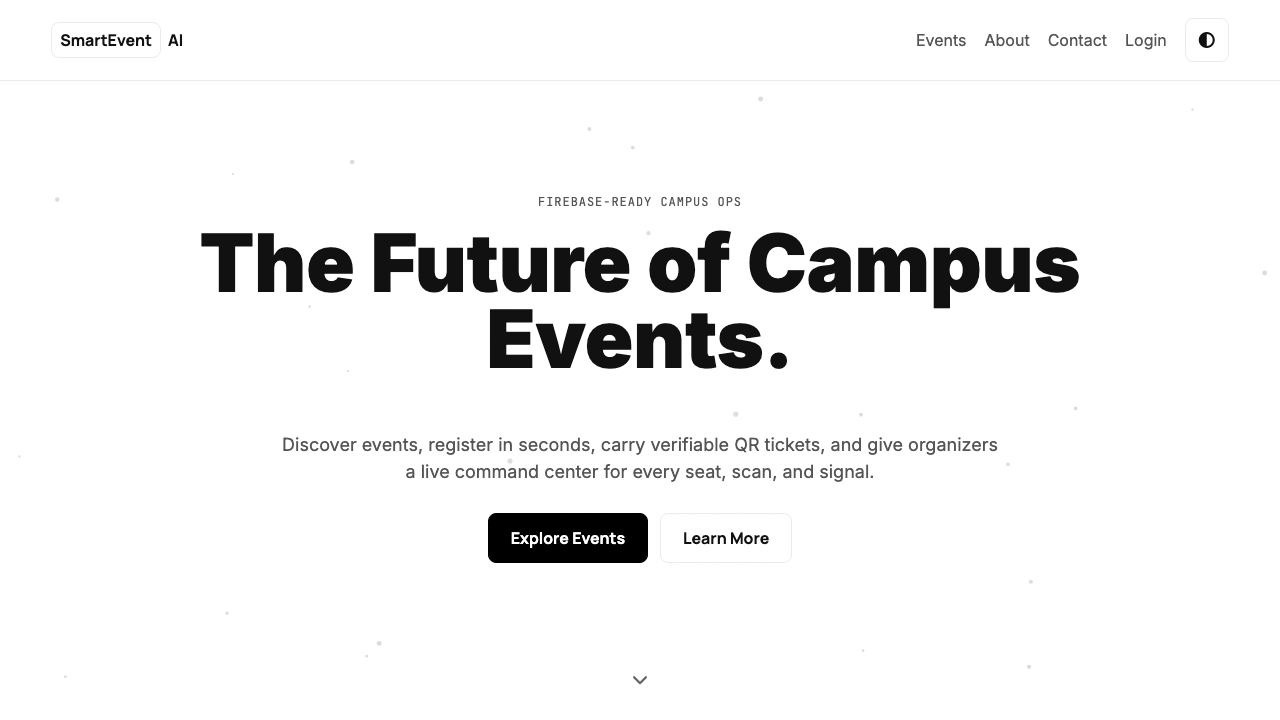
\includegraphics[width=0.9\textwidth]{screenshots/fresh_home.png}
    \caption{SmartEvent AI Home/Landing Dashboard View}
\end{figure}

\vspace{1cm}

\begin{figure}[H]
    \centering
    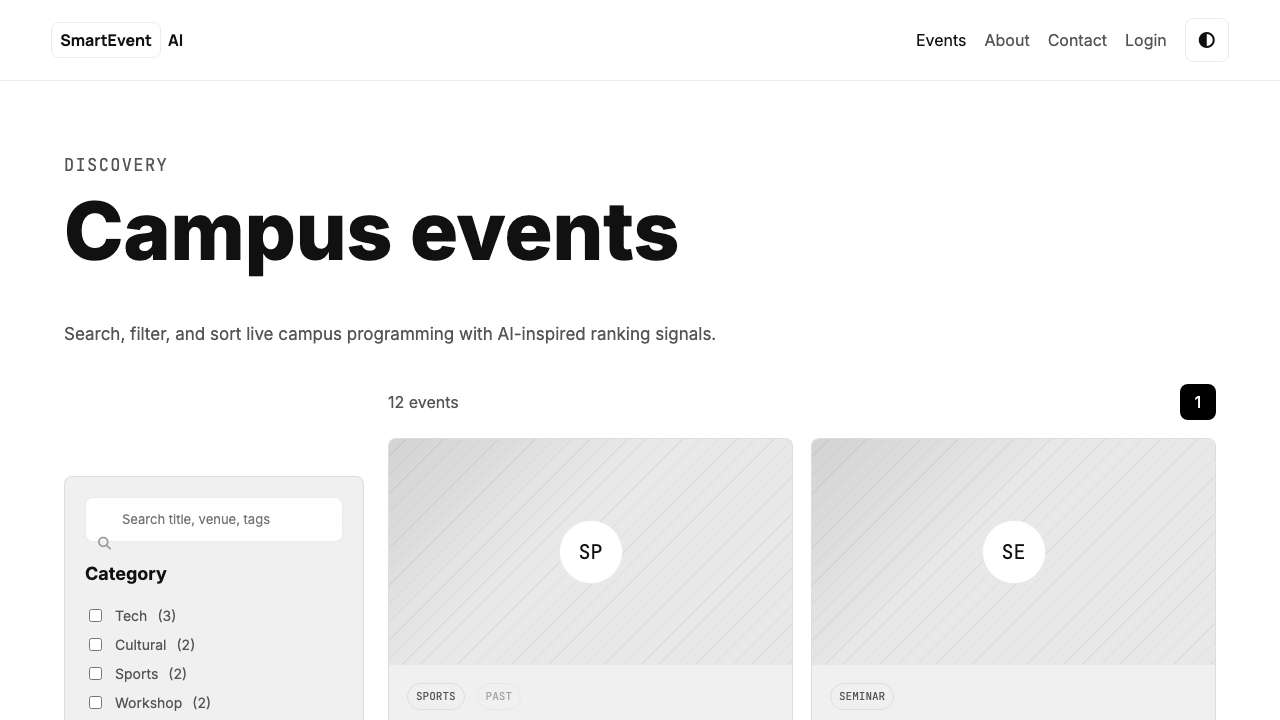
\includegraphics[width=0.9\textwidth]{screenshots/fresh_events.png}
    \caption{Interactive Event Listings Browser with Category Filtering}
\end{figure}

\clearpage

\begin{figure}[H]
    \centering
    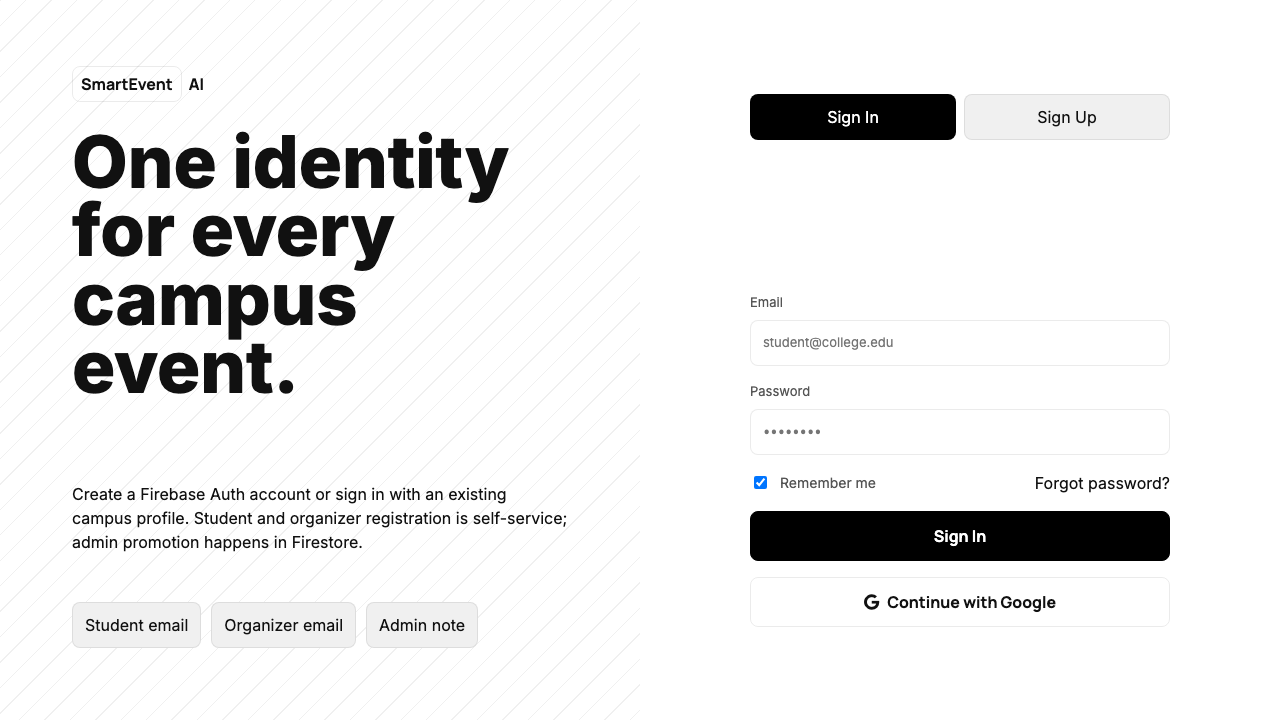
\includegraphics[width=0.9\textwidth]{screenshots/fresh_login.png}
    \caption{Clean Modern Authentication Interface}
\end{figure}

\vspace{1cm}

\begin{figure}[H]
    \centering
    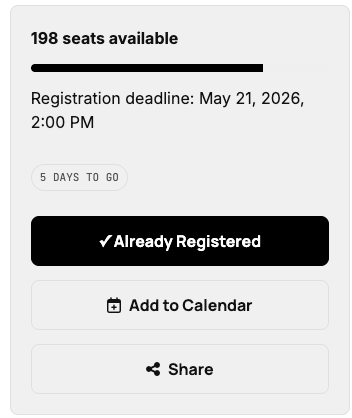
\includegraphics[width=0.45\textwidth]{screenshots/media__1779050121389.png}
    \caption{Reactive Event Detail View with Dynamic Seat Availability \& Progress Bar}
\end{figure}

\clearpage

\section{Database Design}
The database is built on top of Google Cloud Firestore's NoSQL model, optimizing data for rapid read and query speeds. It maintains four core collections:
\begin{enumerate}
    \item \textbf{users:} Holds user account documents identified by their unique Firebase UID. Key fields include: `uid`, `displayName`, `email`, `photoURL`, `role` (student, organizer, or admin), and `createdAt`.
    \item \textbf{events:} Stores event specifications. Key fields include: `id`, `title`, `description`, `venue`, `date` (ISO date), `category`, `totalSeats`, `seatsAvailable`, `registrationCount`, `organizerId`, and `tags` (string array).
    \item \textbf{registrations:} Documents representing active tickets. Key fields include: `id`, `userId`, `eventId`, `ticketId` (randomly generated UUID), `status` (active, attended, or cancelled), and `registeredAt`.
    \item \textbf{attendance:} Audit log for check-ins. Key fields include: `ticketId`, `userId`, `eventId`, `scannedAt`, and `scannedBy` (UID of the scanning organizer).
\end{enumerate}

\section{Implementation Details}
\subsection{Reactive Client State (`SmartStore`)}
The `SmartStore` is the heartbeat of the client-side code. It provides `getState()`, `setState()`, and updates reactive sub-views by dispatching custom window events. This decouples our presentation components from standard state modification loops.

\subsection{WebRTC Camera QR Code Scanning}
To execute live verification, `admin.js` dynamically initializes the device's camera using:
\begin{verbatim}
navigator.mediaDevices.getUserMedia({ video: { facingMode: "environment" } })
\end{verbatim}
The video stream is loaded directly into an invisible `<video>` element. A looping micro-task running inside `requestAnimationFrame` continuously draws the active video frame onto a hidden `<canvas>` context using `drawImage()`. The raw image pixel data buffer is extracted via `getImageData()` and processed through the `jsQR` engine. If a valid ticket UUID is parsed, the scanner triggers an atomic registration lookup. To prevent duplicate scans, the loop pauses for 3 seconds after a successful scan before resetting itself. Furthermore, to avoid battery drain and camera-lock, a DOM listener detects if the user navigates away from the scanner view and calls `.stop()` on all active media stream tracks.

\chapter{TESTING AND RESULTS}
\section{Testing Methodology}
The testing strategy employed a combination of manual verification, regression testing, and stress-testing our reactive state mechanisms:
\begin{itemize}
    \item \textbf{Security Policy Testing:} Authenticated student sessions attempted to make mock POST requests to fetch organizer documents. The database correctly blocked these operations and returned permission errors.
    \item \textbf{Real-Time Synchronization Testing:} We opened two independent browser sessions side-by-side. Registering for an event in window A immediately triggered a DOM update in window B, dynamically decreasing the visual seat counter in real-time.
    \item \textbf{Hardware and Camera Compatibility:} Tested WebRTC video capture across Safari on iOS, Chrome on Android, and desktop devices. Frame decoding latency was verified to be under 200ms across all platforms.
\end{itemize}

\section{Test Cases and Results}
\begin{table}[H]
\centering
\begin{tabular}{|l|p{5cm}|p{5cm}|c|}
\hline
\textbf{Test Case ID} & \textbf{Description} & \textbf{Expected Behavior} & \textbf{Status} \\ \hline
TC-01 & User registration with standard email & User profile created in database with default student role & Passed \\ \hline
TC-02 & Access admin dashboard as student & Page redirects back to home; toast notification shown & Passed \\ \hline
TC-03 & Register for full event & Register button displays "Event Full" and is disabled & Passed \\ \hline
TC-04 & Live QR Scan verification & WebRTC camera scans QR, marks ticket "attended", updates database & Passed \\ \hline
TC-05 & Re-scanning of verified ticket & System flashes toast alerting organizer: "Ticket already scanned" & Passed \\ \hline
\end{tabular}
\caption{System Functional Test Cases and Results}
\end{table}

\chapter{CONCLUSION AND FUTURE WORK}
\section{Conclusion}
The SmartEvent AI project demonstrates that a serverless web architecture provides an incredibly robust, scalable, and lightweight framework for modern collaborative applications. By combining a lightweight Vanilla JavaScript state engine with real-time Firebase services, we constructed a responsive, hardware-free event pipeline. The successfully implemented WebRTC camera-based QR code ticket validator demonstrates that commercial check-in processes can be executed in standard web applications at virtually zero operational cost.

\section{Future Work}
While the platform met all development objectives, several valuable future iterations remain:
\begin{itemize}
    \item \textbf{Offline Sync Capability:} Utilizing service workers and Firestore's offline persistence layer to enable ticket validation even in venues with poor cellular coverage, queuing verification transactions locally until connectivity is restored.
    \item \textbf{Automatic Push Notifications:} Integrating Cloud Functions and FCM (Firebase Cloud Messaging) to dispatch automatic email or push reminders to registered students when an event date is approaching or when an event venue is updated.
    \item \textbf{Payment Portal Integration:} Coupling registration with secure payment gateways (like Stripe or PayPal) to support paid ticketing structures for premium events.
\end{itemize}

\chapter*{APPENDIX}
\addcontentsline{toc}{chapter}{Appendix}

\section*{All Additional UI Screenshots}
The following section contains all remaining screenshots from the development and testing phases of the SmartEvent AI platform.

\begin{figure}[H]
    \centering
    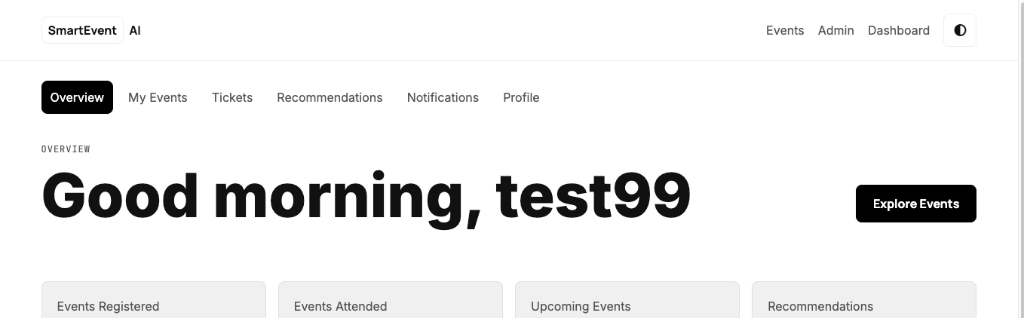
\includegraphics[width=0.8\textwidth]{screenshots/media__1779049052536.png}
    \caption{Create Event Screen (Initial Stretched Layout)}
\end{figure}

\vspace{1cm}

\begin{figure}[H]
    \centering
    
\includegraphics[width=0.8\textwidth]{screenshots/media__1779049124280.png}
    \caption{User Management List (Pre-Firestore Fix)}
\end{figure}

\clearpage

\begin{figure}[H]
    \centering
    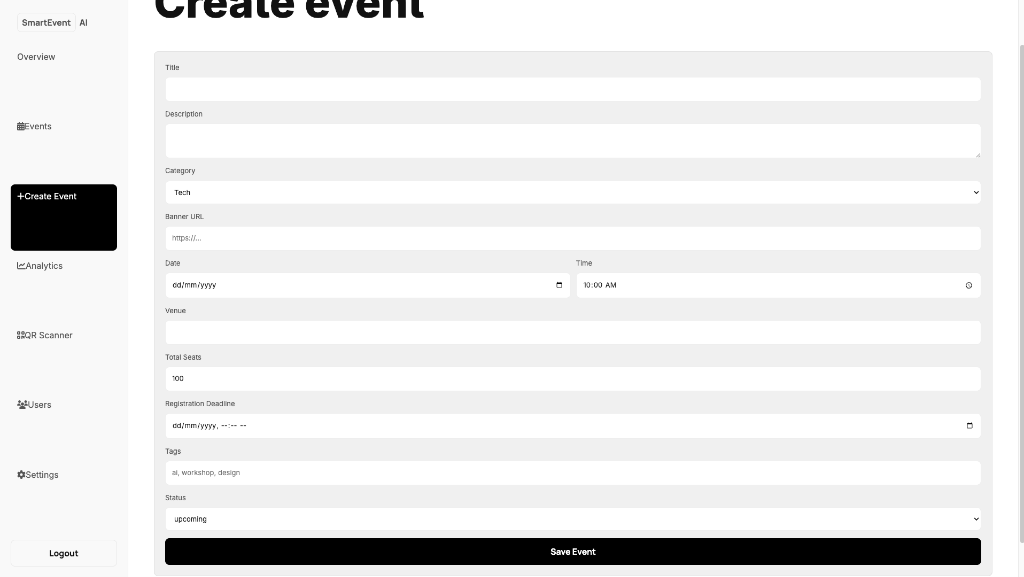
\includegraphics[width=0.8\textwidth]{screenshots/media__1779049508914.png}
    \caption{Create Event Screen (Fixed Max-Width Constraint)}
\end{figure}

\vspace{1cm}

\begin{figure}[H]
    \centering
    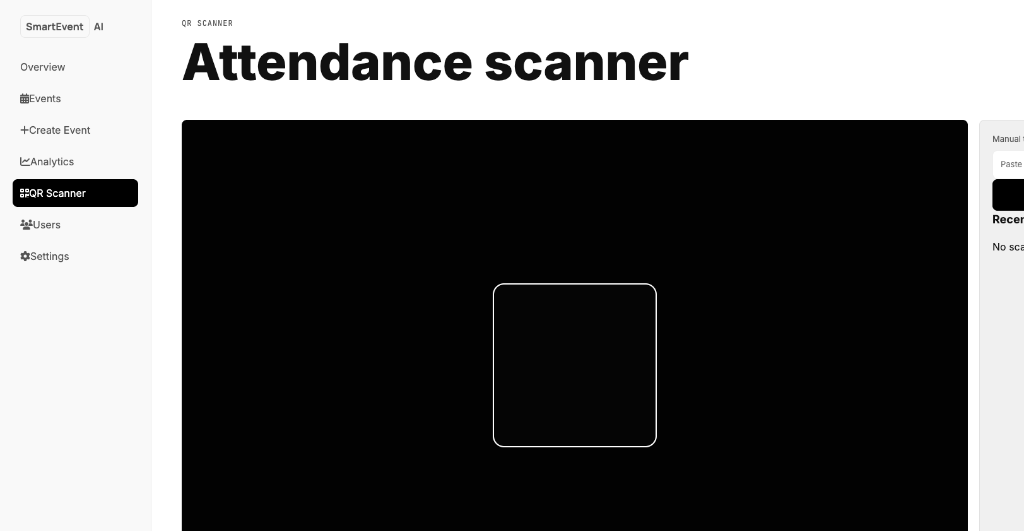
\includegraphics[width=0.8\textwidth]{screenshots/media__1779049852660.png}
    \caption{Event Details Layout Validation}
\end{figure}

\clearpage

\begin{figure}[H]
    \centering
    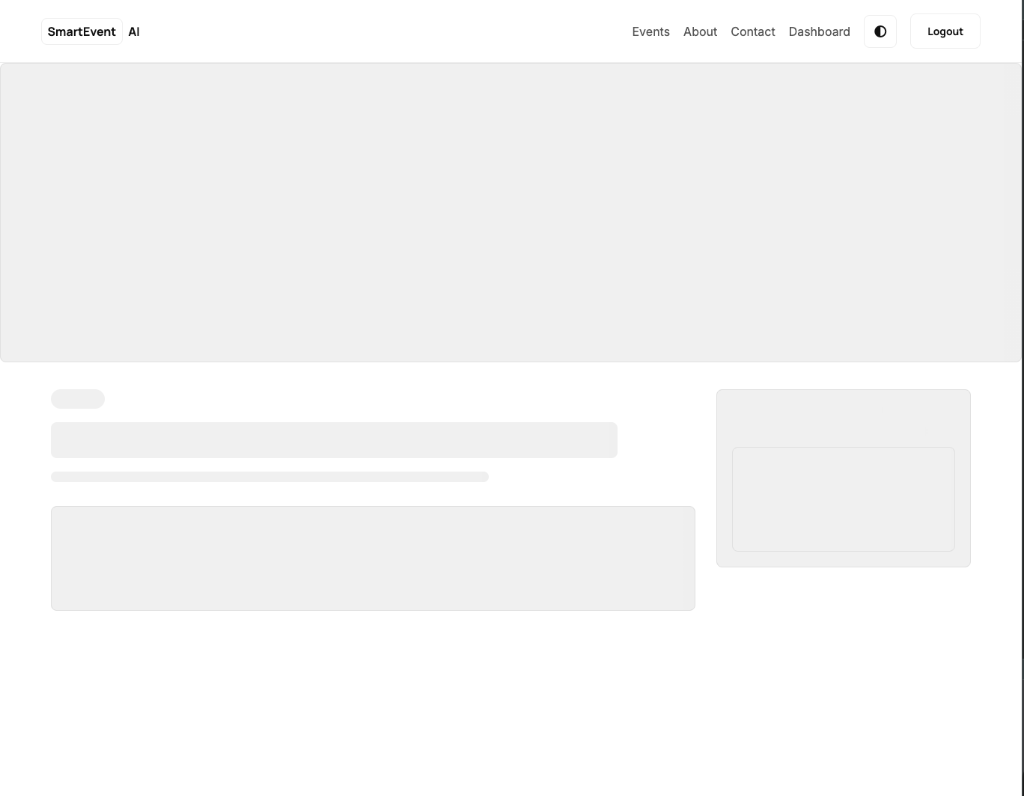
\includegraphics[width=0.45\textwidth]{screenshots/media__1779049984534.png}
    \caption{Interactive Action Panel Component}
\end{figure}

\clearpage

\section*{Source Code}
The complete source code consists of modular JavaScript, Semantic HTML, and custom CSS. The core logic relies heavily on ES6 features and the Firebase v10 SDK.

\section*{GitHub Repository Link}
\url{https://github.com/Ashutoshsingh20/SmartEvent-AI}

\section*{References}
\begin{itemize}
    \item Firebase Documentation: \url{https://firebase.google.com/docs}
    \item WebRTC API: \url{https://developer.mozilla.org/en-US/docs/Web/API/WebRTC_API}
    \item Chart.js Documentation: \url{https://www.chartjs.org/docs/latest/}
    \item jsQR Repository: \url{https://github.com/cozmo/jsQR}
\end{itemize}

\end{document}
